\section{Nuclear Scattering Reactions in the Glauber Framework}\label{sec:reac_model}
Explain path to go:
\begin{itemize}
\item short intro why we use scrattering reactions: to study structure of nuclei (mostly via e. scattering as they only interact via electromagn. force) and refer to chapter. Introduce problems qe account body problem etc
\item starting from elastic scattering at low energies going to medium to high energies
\item explain glauber: eikonal wave approximations, optical limit which leads to optical potential model, description via nucleon nucleon interaction
\end{itemize}
\subsection{Elastic scattering at low energies}
\begin{itemize}
\item Rutherford scattering,poiniering works (alpha particle on gold atoms),description in classical mechanics
\item Rutherford scattering only valid if coulomb potential
\item at low energies below pion production only elastic cross section
\item introduce here the Scattering problem in quantum mechanics (see Schindler, p. 23)
\item from classical physics we go to quantum mechanics and use partial wave decomposition with theta being the scattering angle
\item include in this picture coulomb and nuclear interaction (as done in Kuk, page 120)
\end{itemize}
\subsection{Nuclear Density distribution studies via elastic scattering}
\begin{itemize}
\item Rutherford, Mott and Rosenbluth
\item  show something about form Factors
\item  are charge radii and nuclear radii measured?
\item note approximation for $^{12}C$ that neutron radius same as proton radius
\end{itemize}
\subsection{Glauber Model for nuclear scattering at high energies}
\begin{itemize}
\item explain model assumption
\item eikonal wave approximation: high incoming momentum,low scattering angle
\item Show picture of scattering
\item optical limit: - Nucleons at high energy → undeflected due to large momentum (linear trajectory)
		   -Nucleus large compared to nucleon-nucleon  force
		   -Motion of nucleons independent of nucleus
		   -overall cross-section described in terms of nucleon-nucleon cross section
\item Description in the Probability Approach (also here I use all the eiconal and optical limit approximation)
\item Description in the Eikonal optical-limit approximation
\item Comparison of both descriptions methods  for total interaction cross section,should end up with same. Advantage of PA is that you can calculate the cross section for a defined number of removed projectile nucleons (Schindler, p. 49)
\end{itemize}
\subsubsection{Extensions to the Glauber model}
\begin{itemize}
\item things which cannot be neglected and influence the cross section
\item in medium modifications (see Lukas thesis)
\item Coulomb interaction
\item Pauli blocking
\end{itemize}
\subsection{Cross sections for $^{12}C + ^{12}C$}
\begin{itemize}
\item Total reaction cross section
\item charge changing cross section;maybe I have to include lise++ calculations
\item isotope corrections- neutron removal; maybe I have to include lise++ calculations
\end{itemize}

\subsection{Quasi-Free Scattering (QFS) Reactions}\label{sec:qfs_theo}
Quasi-free scattering (QFS) reactions, as a subset of direct reactions, are processes where a projectile nucleon interacts with a target nucleon via the strong nuclear force in a single and fast localized event at large momentum transfer which allows for a highly localized vertex. The relative kinetic energies of the participants, typically in the order of  $E_{kin}\gtrsim$ 100 AMeV, are high\footnote{Which is needed for the single nucleon-nucleon interaction.The \textit{de Broglie wavelength} of a 100 MeV proton corresponds to $\lambda \approx 2.79fm$ which is in the order of the proton diameter ($\approx 1.6 fm$)}.\newline
In QFS experiments conducted in direct kinematics, a proton serves as the projectile, colliding with a nucleon or a cluster within the target nucleus. Conversely, in inverse kinematics, the nucleus of interest becomes the projectile, while a proton or proton-like particle is used as the target. Despite these differing setups, both approaches are fundamentally equivalent, differing only due to a Lorentz transformation of the reference frame.\newline
As the name implies, QFS reactions are conceptually similar to free nucleon-nucleon scattering, with the primary approximation being that the influence of the residual nucleus is neglected to first order. This approximation simplifies the theoretical description of the process, allowing to treat the interaction as a two-body problem within a (only weakly interfering) nuclear environment.\newline
The first experiments confirming the existence of quasi-free scattering processes were conducted at the University of California, Berkeley, in 1952 by O. Chamberlain and Emilio Segr\`e\cite{chamberlain1952proton}. In their study, lithium nuclei were bombarded with 350 MeV protons, and coincident proton pairs were observed with an opening angle of approximately 90$^{\circ}$. That same year, J.B. Cladis, W.N. Hess, and B.J. Moyer published results on the scattering of 340 MeV protons on deuterium and carbon targets\cite{cladis1952nucleon}, further substantiating the phenomenon.\newline
In 1957, Tyr\'en, Maris, and Hillman designed an experiment aimed at fully characterizing proton-proton collisions within the quasi-free scattering framework\cite{MARIS19581}. Their results validated the assumption of a direct and clean interaction between the projectile and the target nucleon, free from significant distortions caused by the surrounding nucleus. Furthermore, these experiments demonstrated that QFS reactions could serve as a powerful tool for probing nuclear structure and testing predictions of the shell model. Specifically, they enabled the study of key nuclear parameters such as spin-orbit splitting and energy differences between nuclear shells probing the shell evolution. \newline
In QFS reactions, these parameters can be extracted by analyzing the reaction products, which include the two correlated outgoing protons, the residual nucleus, and any gamma rays emitted during de-excitation of the residual nucleus. The detailed measurements of these observables provide critical insights into the underlying nuclear structure and dynamics.\newline
The experimental discoveries and theoretical insights from these early studies strongly pushed the advancements in the theoretical modeling of QFS reactions. These models have since become essential tools for understanding nucleon-nucleon interactions within the nuclear medium and for further investigations of nuclear structure and reaction mechanisms.\newline
\subsubsection{Kinematics of QFS Reactions}\label{sec:kin_qfs}
A simplified picture, which however explains the essential kinematics of the QFS reaction, can be found in figure \ref{fig:sketch_qfs}: we have an incoming proton knocking out a nuclear constituent (proton/neutron) in a quasi-free nucleon-nucleon collision ending with a final state having the scattered proton, the scattered  off nuclear constituent and the rest nucleus (A-1), which could be either in the ground-state or an excited state. In this picture index \textit{0} is assigned to the incoming proton, \textit{1} to the knocked out nucleon, \textit{2} to the outgoing projectile proton, \textit{A} to the initial nucleus and  \textit{A-1} to the final nucleus accordingly.
\begin{figure}[htpb]
    \centering
    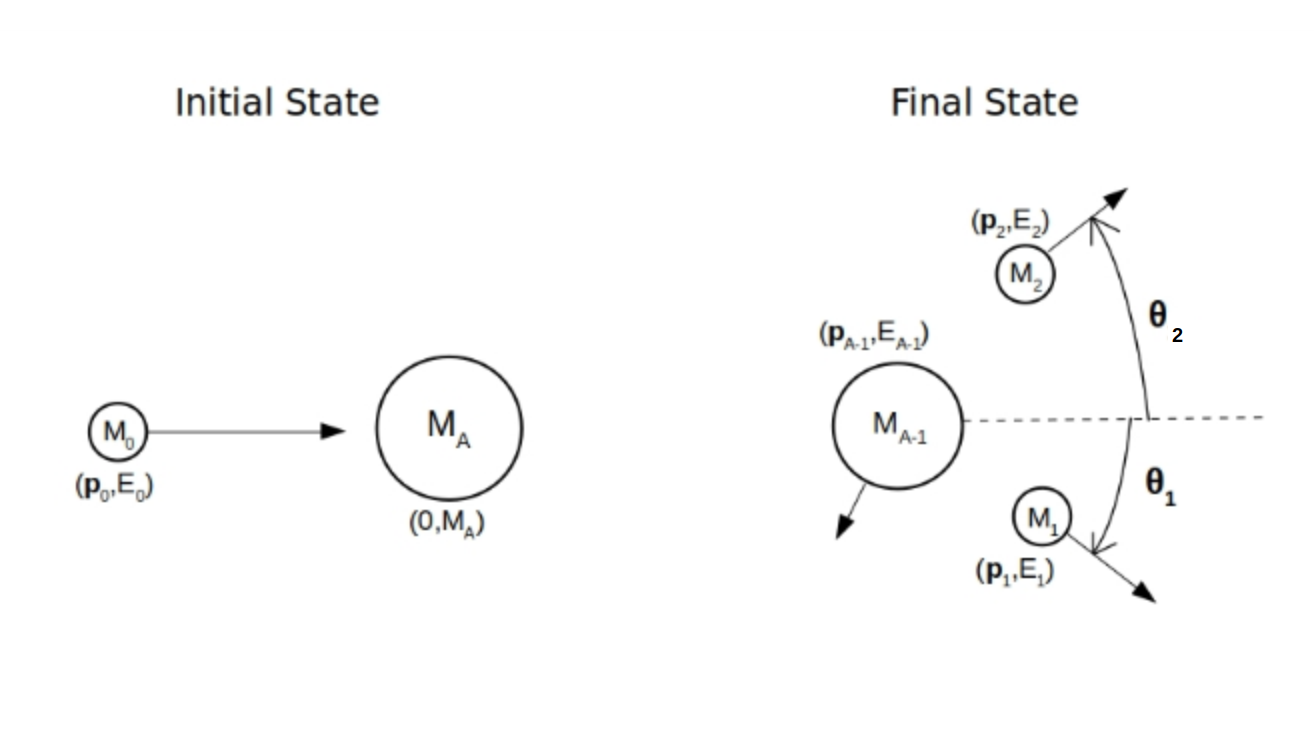
\includegraphics[width=\textwidth,height=8cm,keepaspectratio=true]{Figures/sketch_qfs.png}
    \caption{
   	Simplified picture of the QFS reaction process in direkt kinematics.  
    }
    \label{fig:sketch_qfs}
\end{figure}
As from standard textbooks (see~\cite[Chapter~6.2]{povh2013teilchen}) the energy-momentum conservation of the reaction can be expressed as:
\begin{equation}\label{eq:four_mom_cons_qfs}
P_A  +  P_0 = P_1 + P_2 +P_{A-1} 
\end{equation}
with $P_i$ the four momentum $(E_i,\mathbf{p_i})$.\newline
In direct kinematics as presented in figure \ref{fig:sketch_qfs} the separation energy  of the ejected nucleon for a certain final state of the nucleus \textit{A-1} is given by\footnote{In inverse kinematics the four-momentum vectors need to be boosted to the center of mass frame of the initial nucleus via Lorentz transformation.}:
\begin{equation}
S = T_0 -(T_1+T_2 +T_{A-1}); \; \text{with $T_i$ the kinetic energy of particle $i$} 
\label{eq:sep_e}
\end{equation}
In the idealized shell model the separation energy equals to the (negative) energy of the nucleus' single-particle state. In the case where the final nucleus \( A-1 \) (corresponding to a one-proton knockout) remains in its ground state, its total energy in the center-of-mass frame of the initial nucleus is given by
\begin{equation}
E_{A-1} = M_{A-1}c^{2} + T_{A-1},
\end{equation}
where \( M_{A-1} \) denotes the rest mass of the final nucleus and \( T_{A-1} \) its kinetic energy after the quasi-free nucleon-nucleon collision.\newline
If a nucleon has been ejected from an inner shell resulting in a hole state, the final nucleus will be in an excited state:
\begin{equation}
E^{*}_{A-1} =  M_{A-1}c^2  +T_{A-1} + E_{exe}
\end{equation} 
From the experimental point of view $E_{exe}$ is directly accessible via gamma detection from the transition of the final nucleus from the excited to the ground state or via the detection of evaporated neutrons from higher excited states.\newline
From momentum conservation follows that in the center-of-mass frame of the initial nucleus ($\mathbf{p_A} = 0$), the recoil momentum of the nucleus in final state $\mathbf{p_{A-1}}$ equals to $-\mathbf{p_i}$, the momentum of the initial nucleon inside the nucleus A pointing in opposite direction. \newline
In addition the four-momentum of the inner nucleon can be deduced from momentum measurement of the initial and final state free nucleons:
\begin{equation}\label{eq:miss_mom}
P_i \approx P_{miss} \equiv P_1 + P_2  - P_0
\end{equation}
where $P_{miss}$ is the so called "measured missing four-momentum of the reaction"\cite{patsyuk2021unperturbed}\footnote{$P_{miss}$ is only equal to $P_i$ for the unperturbed QFS (no ISI/FSI) case.}.
Thereupon, the separation energy measurement and the recoil momentum distribution fully describe the single paricle state in the various shell levels. 
In addition and as complementary method $\gamma$ rays can be measured in coincidence with the reaction and consequentely exclusive cross section and momentum distribution measurements of the single particle states are accessible.\newline
Considering the removal of a single nucleon from an initial nucleus state $\Psi^A_i$ with A nucleons and initial spin \textit{I} and final nucleus state  $\Psi^{A-1}_f$ with final spin $I_f$ an overlap function between intial and final state many-body wave function can be written as:
\begin{equation}
\langle \vec{r}, \Psi_f^{A^{-1}} | \Psi_i^A \rangle = \sum_j C_j^{if} \psi_j(\vec{r}), \quad with  |I - I_f| < j < |I + I_f|
\end{equation}
where $S_j^{if} = |C_j^{if}|^2$ is the commonly named spectroscopic factor, see ref \cite{hansen2003direct} sec.2.1. $S_j^{if}$ is summed over all final single particle states m (from $-j$ to $j$). It is unity for nucleon removal from a pure single particle state and in this picture equals (2j+1) when the nucleon was removed from a filled j-subshell.
In a more realistic model the spectroscopic factor is linked to the exclusive experimental cross section measurement of a single particle state $\sigma_{sp}(nlj)$ and the theoretical predicted one, as in ref \cite{hansen2003direct}:
\begin{equation}
\sigma_{th}^{if} = \sum_j S_j^{if}\,\sigma_{sp}(nlj)
\end{equation}
where $\sigma_{sp}$ are the theoretical cross sections for the normalized wave functions $\Psi_j$ of the final state nucleus A-1 with the appropriate quantum numbers.\newline
From this considerations the spectroscopic factor can be used to probe the theoretical shell predictions. In past this was already done with direct QFS-reactions $(e,e'p)$. Results for the spectroscopic factor with data obtained at the NIKHEF facility are shown in figure \ref{fig:spec_fac}. The substantial reduction of the spectroscopic factor with respect to the independent particle model (IPM) or mean field of $\approx 35\%$ indicates a substantial depletion of the single-particle states and inferring from this a refined model prediction has to be applied\footnote{The mean field potential does not consider spin-spin interaction $V_{ss}$, non central tensor-potential $V_T$ or spin-orbit interaction $V_{LS}$.}.\newline
\begin{figure}[h!]
    \centering
    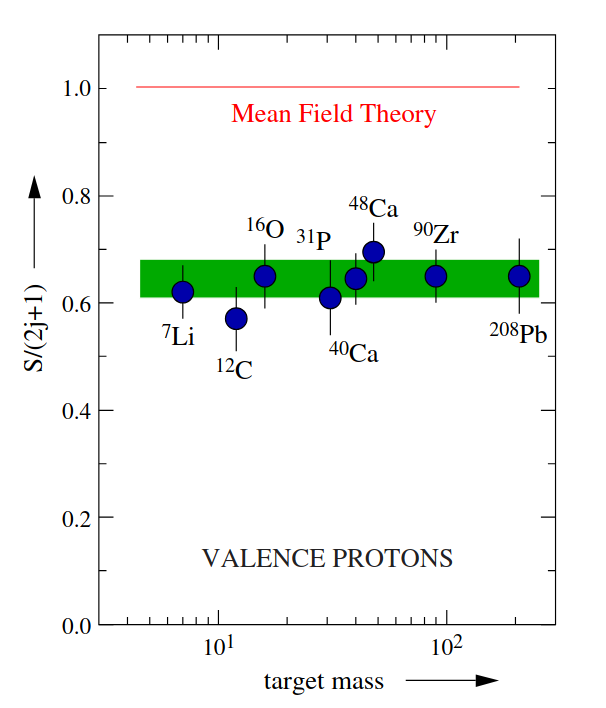
\includegraphics[width=\textwidth,height=8cm,keepaspectratio=true]{Figures/spec_factor.png}
    \caption{Normalized spectroscopic factors from the $(e,e'p)$ reaction as a function of target mass taken from \cite{DICKHOFF2004377}. As input for the theoretical cross sections the prediction from mean field models were used. }
    \label{fig:spec_fac}
\end{figure}
While QFS-reaction with electrons $(e,e'p)$ in direct kinematics is a valuable method to make precise measurements for stable (target) nuclei it is not suitable for the experimental analysis with exotic (neutron or proton rich) nuclei. Due to their short lifetime (e.g. $^{52}Ca$ with $\tau = 4.6s$) they can hardly serve as a target. Inducing the reaction in inverse kinematics - having electrons as targets and the exotic nuclei of interest as projectiles - is also not feasible since no free electons can be captured as target and even more important the required center of mass energies in such an asymmetric system would require extremely high beam energies. The alternative approach is to use proton induced quasi-free scattering in inverse kinematics where the exotic beam inpinges on an extended proton target such as liquid hydrogen $H_2$  or a fixed proton rich target such as $CH_2$\footnote{Herefore a carbon target reference run is used to extract the QFS-reaction events from the $CH_2$ target run.}.\newline
Summarizing, the QFS-reaction technique in inverse kinematics with exotic nuclei as in-flight projectiles and a proton-like target opens new possibilities to probe theoretical model predictions of exotic nuclei far off stability which haven't been accessible before.\newline
For precise cross section measurements of the single particle states $\sigma_{sp}$ the kinematical characteristics of the QFS-reaction products have to be considered for correct identification of QFS-events and clear background substraction. The following descriptions are already implicitly embedded within the equation \ref{eq:four_mom_cons_qfs}.\newline
As starting point one compares the QFS-reaction of the two nucleons with the two dimensional non-central collision of free pointlike particles in nonrelativistic kinematics. Since both kinetic energy and momenta are conserved a  clear signature is expected: the opening angle of the scattered particles is exactly 90$^{\circ}$. 

However, at kinetic energies of 400 AMeV and more, relativistic effects affect the opening angle of the scattered particles\footnote{Relativistic considerations become relevant at velocities $ \beta \gtrapprox 0.1 c$. This corresponds to $\approx$ 4.5 MeV.}. 
TODO: Formula to calculate directly from beam energy the opening angle...

For the final description of the process it has to be considered that the projectile nucleon inside the nucleus has a non negligible momentum (see $P_i$ in equation \ref{eq:miss_mom})  and in addition the separation energy $S_{p/n}$ has to be expended to remove the scattered nucleon of the nuclear potential of the projectile nucleus.\newline
To account for the nucleon momentum the picture of the fermi gas model where protons and neutrons freely move inside the nucleus' potential is applied. In the ground state of the nucleus the nucleons can reach a momentum up to the Fermi momentum $p_F$. Except for the light nuclei, the Fermi momentum is almost independent of A and amounts to $ p_f \approx 250$ MeV/c \footnote{For light nuclei like $ ^{12}C$, $p_F \approx 230$ MeV/c can be assumed~\cite{moniz1971nuclear}}. The mean quadratic momenta of the nucleons is related to the Fermi momentum by:
\begin{equation}
\langle \mathbf{p}^2 \rangle = \frac{3}{5}p^2_F \footnote{From the derivation of the mean kinetic energy of the nucleons $\langle E_{\text{kin}} \rangle = \frac{\int_0^{p_F} E_{\text{kin}} \, p^2 \, dp}{\int_0^{p_F} p^2 \, dp} = \frac{3}{5} \cdot \frac{p_F^2}{2M}$}
\end{equation}
The width of the momentum distribution of the nucleons is given in the Goldhaber model by:
\begin{equation}
\sigma^2 = \sigma_0^2 K(A-K)/(A-1), \, \text{with} \, \sigma_0 \approx 90 MeV/c
\end{equation}
where A is the mass number of the projectile nucleus and K the mass number of the fragment after scattering. For a detailed derivation and further readings see ref. \cite{goldhaber1974statistical} and \cite{FESHBACH1973300}.
In the impuse approximation, where we assume that the interaction between the projectile and target nucleons has approximately the same form as the interaction between two nucleons in free space, the inner momenta of the scattered nucleons smear out the angular correlations of the outgoing fragment - which has the same momentum as the knocked out nucleon in the cms system of the nucleus but points in opposite direction - as well as of the two nucleons involved in the scattering. As consequence the opening angle distribution of the two scattered nucleons gets broadened as well as the azimuthal angular correlation which for the assumption of zero nucleon momentum sharply peaked at $\Delta\varphi = 180^{\circ}$.\newline
In view of the added nucleon momentum the kinematics get expanded from a two dimensional scattering reaction to a three dimensional process where the reaction plane is determined by the plane spanned by the momentum vector of the projectile nucleus $\mathbf{p}_A$ and the scattered nucleon after the reaction \footnote{For (p,2p) reactions there is an ambigousity which of the scattered protons $\mathbf{p}_1$ or $\mathbf{p}_2$ origin from the projectile nucleus or the proton like target.}. With the momentum measurement of the two correlated outgoing nucleons and the momentum of the incoming projectile nucleus it is possible to retrieve the internal momentum of the knocked out nucleon perpendicular to the reaction plane $Q_{\perp i}$ via the formula derived in reference\cite{chulkov2005quasi}:
\begin{equation}\label{eq:chulkov}
Q_{\perp i} = sin(\theta_{1/2})\cdot sin(\varphi_{1/2} -\varphi_{2/1})\cdot\mathbf{p}_{2/1}
\end{equation}
In case of (p,2p) reactions it is impossible to track back the origin of each nucleon - from the projectile nucleus or the proton-like target. Inferring from this there are two possible solutions for $Q_{\perp}$. The ambiguity can be resolved by incorporating the momentum of the fragment nucleus perpendicular to the reaction plane $Q_{\perp A-1}$. The fragment momentum vector should be of the same amout but point in opposite direction to $Q_{\perp i}$.
TODO: maybe insert here the plot of $Q_{\perp}$ if possible...

Up to this point, the scattering process has been described analogously to free elastic scattering in relativistic kinematics, with the knocked-out nucleon assumed to possess a non-negligible initial momentum inside the nucleus. However, it must be noted that the ejected nucleon is an off-shell particle, bound within the nuclear potential. Its virtual mass \( \mu_i \) in the c.m.s. of the nucleus is given by:
\begin{equation}
\mu_i =  \sqrt{m_A^2 + m_{A-1}^2 - 2m_A\sqrt{m_{A-1}^2 + |\mathbf{p}_i|^2}}
\label{eq:virtual_mass}
\end{equation}
where \( m_A \) and \( m_{A-1} \) are the rest masses of the initial nucleus and the residual fragment after the quasi-free scattering, respectively, and \( \vec{p}_{i} \) denotes the momentum of the inner nucleon  in the c.m.s. of the nucleus, see also equation \ref{eq:miss_mom}. From equation \ref{eq:virtual_mass} follows:
\begin{equation}
0 < \mu_i  < m_n
\end{equation}
where $m_n$ is the mass of the appropriate free nucleon.
To knock the bound nucleon out of the nucleus the separation energy has to be overcome which can be observed in the reduced opening angle of the two outgoing correlated nucleons.



%From experimental point of view-> important to identify the QFS events.
%In non rel. kinematics of free particles a really clean signature: two dim-colllision with coplanar nucleons = delta phi = 180 degr and an opening angle of 90 degr. \newline
%When going to rel. energies -> 80 degrees of opening angle(400 AMeV). Is there a function to calculate the opening angle? The opening angle is smeared because of relativistic effects + inner momentum of the nucleon. \newline
%Explain Goldhaber model to characterize the width of the inner momenta.\newline
%Plot the correlation plots of opening angle and delta phi.
%Then mentnion pronounced transversal correlation as in L.V. Chulkov -> insert image
%Moreover limited energy ranges are allowed where the forward nucleon has much higher energy compared to the larger scattered one -> insert image
%

\subsubsection{Cross Sections for QFS Reactions - Qualitative Considerations}
TO DO: see more in the standard work \cite{cladis1952nucleon}, \cite{MARIS19581}.
\subsubsection{Application Fields of QFS Reactions}
Over several decades of experimental and theoretical research, Quasi-Free Scattering (QFS) reactions have been firmly established as a powerful and direct tool for probing the microscopic structure of atomic nuclei. These reactions provide critical insights into nuclear correlations, single-particle properties, and the momentum distributions of nucleons within the nucleus.\newline
The versatility of QFS extends across various applications, including the study of short-range nucleon-nucleon interactions, exotic nuclear states, and the modification of nucleon properties in nuclear matter. Advances in experimental facilities and state-of-the-art detector systems, have significantly improved the precision and scope of QFS measurements. These developments have enabled in-depth investigations of nuclear dynamics, the structure of unstable isotopes, and fundamental aspects of quantum many-body systems, contributing to a deeper understanding of nuclear and subnuclear phenomena.\newline
This subsection will point out the most exciting and promising application fields of QFS reactions with focus on the applicability in the R$^3$B experimental setup. A detailed review can be found in ref \cite{panin2021quasi}.
\begin{description}
\item[Single-Particle Spectroscopic Strength]As already mentioned in section \ref{sec:kin_qfs} in many experiments a reduction in the spectroscopic strength of about 35\% with respect to the independent particle model (IPM) and shell model predictions was observed. In one-nucleon removal reactions - experiments with isotope beams impinging on a composite nuclear target - the extraction of the missing spectroscopic strength is challenging as the kinematical pattern is highly complex. In contrast, the QFS reactions mechanism in inverse kinematics retains a clear kinematical signature which makes it a valuable tool to study the quenching of the spectroscopic strength which originates from residual correlations between bound nucleons inside the nucleus. \newline
Several experiments were carried out at the GSI Facility to study the reduction factor of the spectroscopic strength  and its evolution over a broad range in isotopic chains, in light nuclei such as for oxygen shown in figure \ref{fig:red_factor}. With the commmissioning of the SIS100 and SuperFRS at GSI it will be achievable to study (p,2p) reactions with very short lived nuclei also in heavier systems at reasonable intensities which will presumably draw even more attention to QFS reaction approach.  
\begin{figure}[htpb]
    \centering
    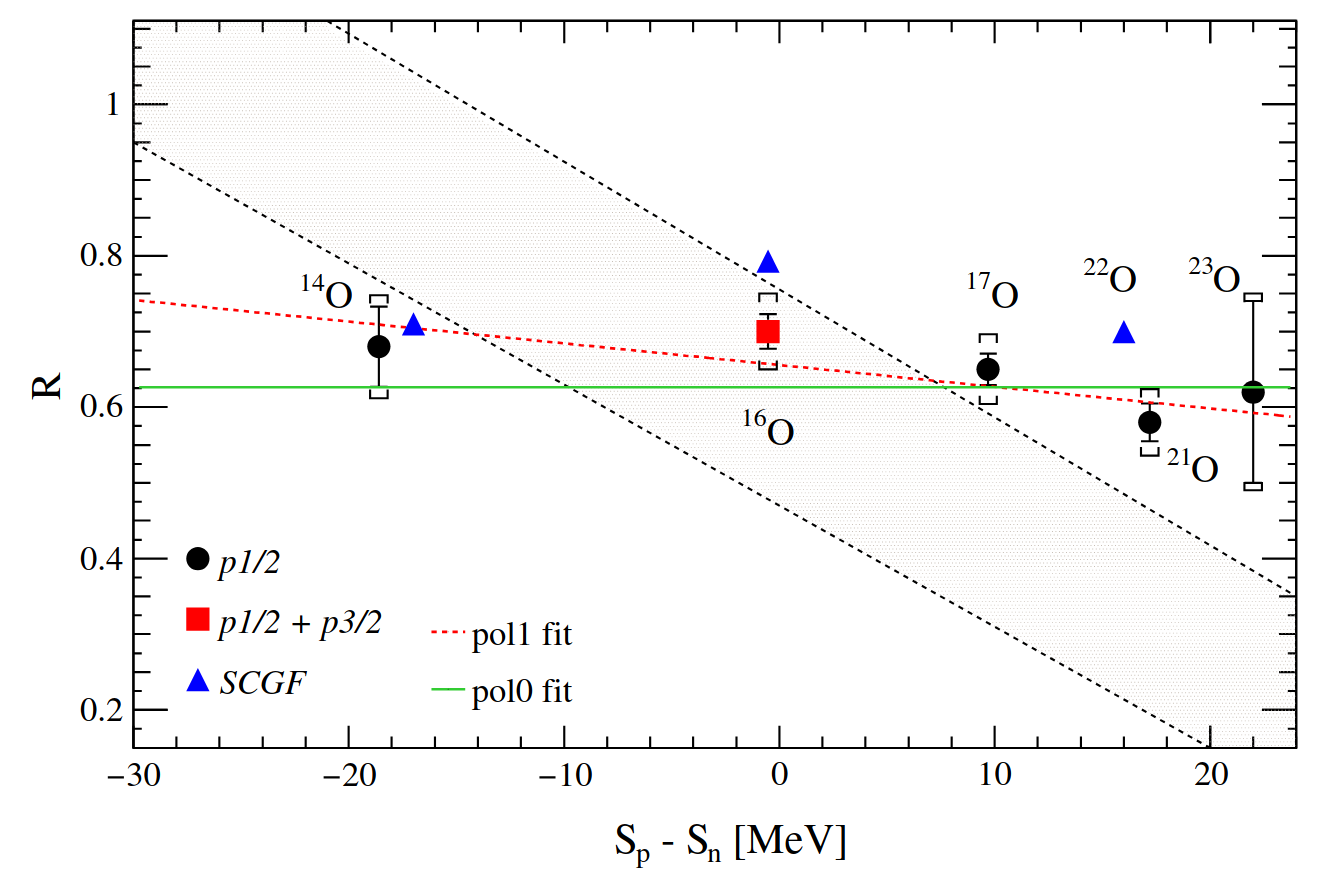
\includegraphics[width=\textwidth,height=8cm,keepaspectratio=true]{Figures/spec_red_factors.png}
    \caption{
   	Extracted reduction factors of the spectroscopic strength from (p,2p) measurements (circles and square) as a function of the difference between proton and neutron separation energy $S_p$/$S_n$. The blue triangles correspond to the predictions from self-consistent green functions (SCGF). The shaded area indicates a trend from an analysis of one-nucleon removal cross sections in other reactions and which lead to an intense discussion in the field. From Ref. \cite{atar2018quasifree}.   
    }
    \label{fig:red_factor}
\end{figure}
\item[Gamma Spectroscopy]Alongside to the study of the single-particle spectroscopic strengths QFS reactions provide valuable information of the shell structure and deformation of the fragment (A-1) via gamma spectroscopy. QFS reactions with nucleons in inner shells result in bound (or unbound) excited states of the (A-1) fragment. The excited fragment promptly decays to its ground state either through the emission of a Doppler-shifted \(\gamma\)-ray, or -- if the excitation energy exceeds the particle separation threshold -- via the emission of a proton or neutron.\newline
A big advantage of the (p,2p) reaction experiments is the ability to make precise vertex reconstruction by accurate measurement of the two outgoing correlated protons. This is of particular importance for extended targets and determines the emission point within the target, enabling an accurate calculation of the fragment's velocity and therefore a precise Doppler correction.\newline
From gamma spectroscopy the excitation energy E(2+), often the first excited state in even-even nuclei, can be observed which is a fundamental observable of nuclear structure, providing key insights into the shell configuration and deformation of the nucleus\cite{panin2021quasi}. Expecially when going towards exotic neutron rich isotopes the study of the gamma emission lines can strongly contribute to the understanding of nuclear shell evolution.
\item[QFS to probe inner clustering and halo formation]Clusterization inside nuclei is a phenomenon widely observed in experiments with large implications on astrophysics processes such as the synthesis of carbon  inside stars via triple $\alpha$ clusterization \cite{hjorth2011carbon}, $\alpha$ - radioactivity, or the evolution of core collapse supernovae\cite{sumiyoshi2008appearance}, just to mention some. Its presence has also to be implemented in the state of the art equation of state calculations.\newline
Single-particle cluster states can be directly accessed via QFS (p,p$\alpha$) reactions. In the low energy regime of 100 AMeV the $^{12}\text{C}(p, p\alpha)^{8}\text{Be}$ reaction, see ref \cite{mabiala2009analyzing}, as benchmark study approved the reaction mechanism and up to a scaling factor the measured cross sections aligned exceptionally well to the free p–$\alpha$ scattering measurements.\newline
Moreover the QFS mechanism allows to acces light nuclei going towards the neutron drip line via (p,pn) reaction. These light nuclei are mostly weakly bound with an extended low density neutron-matter distribution forming a so-called \textit{nuclear-halo}.\newline
The most prominent candidate for such is $^{11}Li$, often called \textit{Borromean three-body system}, consisting of two neutrons interacting with a core ($^9Li$) via weak, short-range interactions~\cite{johannsen199011li}. First evidence for the correlation  between the two neutron was strongly pushed by experimental studies at GSI, see \cite{simon1999direct}, and theoretical work by Bertulani et. al.\cite{bertulani2007geometry}.\newline
The latest experiment with the focus on the study of multi-neutron correlations in drip-line nuclei was carried out at R$^3$B in 2022 (experiment S509) probing broad isotopic chains of Li, Be, B, C and N via the QFS mechanism, and first results are expected to be published in the near future.
\item[Short Range Correlations(SRC)]Short range correlations refer to elementary nucleon-nucleon interactions within a nucleus and occur over very short distances, typically on the order of 1-2 femtometers.  These correlations are characterized by pairs of nucleons with high relative momentum ($> k_F$, Fermi momentum) and low total momentum. These NN-interactions are treated as good explanatory candidate for observed deviations from mean field approximation. Many phenomena, such as the above discussed reduction in the spectroscopic strength and the EMC effect\cite{xing2023electromagnetic}, the observation that  the cross section for deep inelastic scattering from an atomic nucleus is different from that of the same number of free protons and neutrons, are associated to the short range correlations inside the nucleus.\newline
From isotopic chain studies\cite{clas2018probing} it has been shown that there is an indication of SRC depenency on isospin, see figure \ref{fig:src_pairs}, where SRC are predominatly preferred by p-n pairs than by nn or pp pairs. This again can have significant impact for asymmetric nuclei and imply a stronger quenching of the spectroscopic strength for proton single particle states below the Fermi momentum for neutron rich matter.\newline  
Since pioneering experiments were made at JLab and Brookhaven via $(e,e'p)$ and $(e,e'n)$ reactions several  experimental campaigns were carried out at GSI with the R$^3$B setup probing the QFS reactions via the strong nuclear forceinstead of the Coulomb interaction. Also in 2022 the S522 experiment was performed to exploit for the first time the use of short-lived nuclei scattering off a proton probe in inverse kinematics at R$^3$B, followed by the S091 experiment in 2024 with the focus on probing NN-correlations in atomic nuclei via $(p,pd)$ QFS reactions\cite{paschalis2020nucleon}. 
\begin{figure}[htpb]
    \centering
    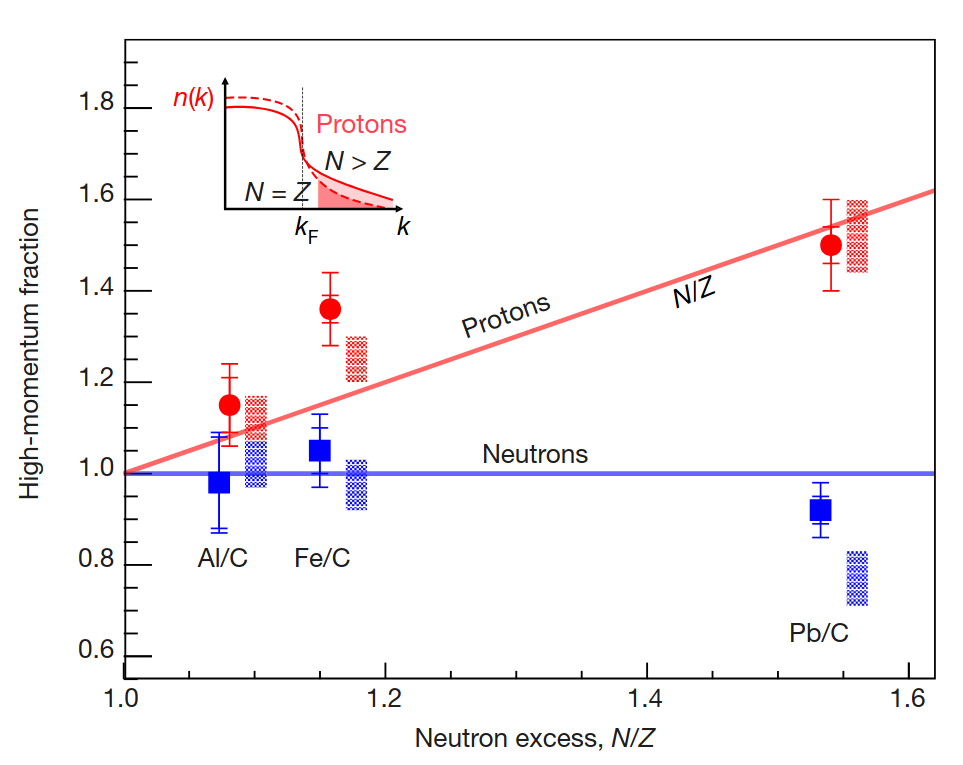
\includegraphics[width=\textwidth,height=8cm,keepaspectratio=true]{Figures/src_pn_excess.png}
    \caption{
   	Fraction of high-momentum neutrons and protons with respect to the N/Z ratio for several carbon isotopes. A clear trend towards high momentum proton distribution for neutron rich carbon isotopes (red line) is shown, while the high momentum neutron distribution stays constant wiht respect to the N/Z ratio (blue line). From reference \cite{clas2018probing}. 
    }
    \label{fig:src_pairs}
\end{figure}

\end{description}

\subsubsection{QFS and Coulex: A Complementary Approach to Fission}
Fission induced via quasifree scattering (QFS) provides a powerful method to extract fission barriers on an event-by-event basis. The fundamental concept involves the knockout of a proton or neutron from an incoming exotic ion beam. By measuring the energy  and the angular distribution of the correlated emitted nucleons, it becomes possible to probe the excitation energy transferred to the fissioning system. In cases where deeply bound nucleons are knocked out, the resulting daughter nucleus either evaporates one or multiple neutrons or populates an excited state, which can be experimentally observed. The R$^3$B setup is particularly well-suited for such investigations, as it enables full kinematic reconstruction of the reaction products and hence to pin down the complete reaction mechanism. This approach allows for the detailed exploration of the potential-energy surface and the fission dynamics across a broad range of fissility and excitation energies, taking advantage of relativistic radioactive beams.\newline
The pilot experiment S455 was conducted in 2021 at R$^3$B using a stable $^{238}$U beam incident on a liquid hydrogen target. The data collected from this experiment provide simultaneous information on several key fission observables, which can be used to constrain theoretical calculations. These calculations aim to describe both the static and dynamic properties of the fission process and enable comparisons with predictions from various theoretical frameworks, including phenomenological approaches, macroscopic-microscopic models, and fully microscopic statistical or time-dependent Hartree-Fock calculations.\newline
A critical aspect of this experimental setup is the simultaneous measurement of the two outgoing fission fragments. This is achieved using a dedicated ionization chamber (TWIM-MUSIC) and advanced tracking detectors. The success of this methodology has already been demonstrated by promising results, see \cite{garcia2023study},\cite{grana2023fission} and figure \ref{fig:qfs_fission}, highlighting the potential of this technique in advancing our understanding of nuclear fission dynamics.\newline
\begin{figure}[htpb]
    \centering
    \begin{subfigure}[b]{0.3\textwidth}
    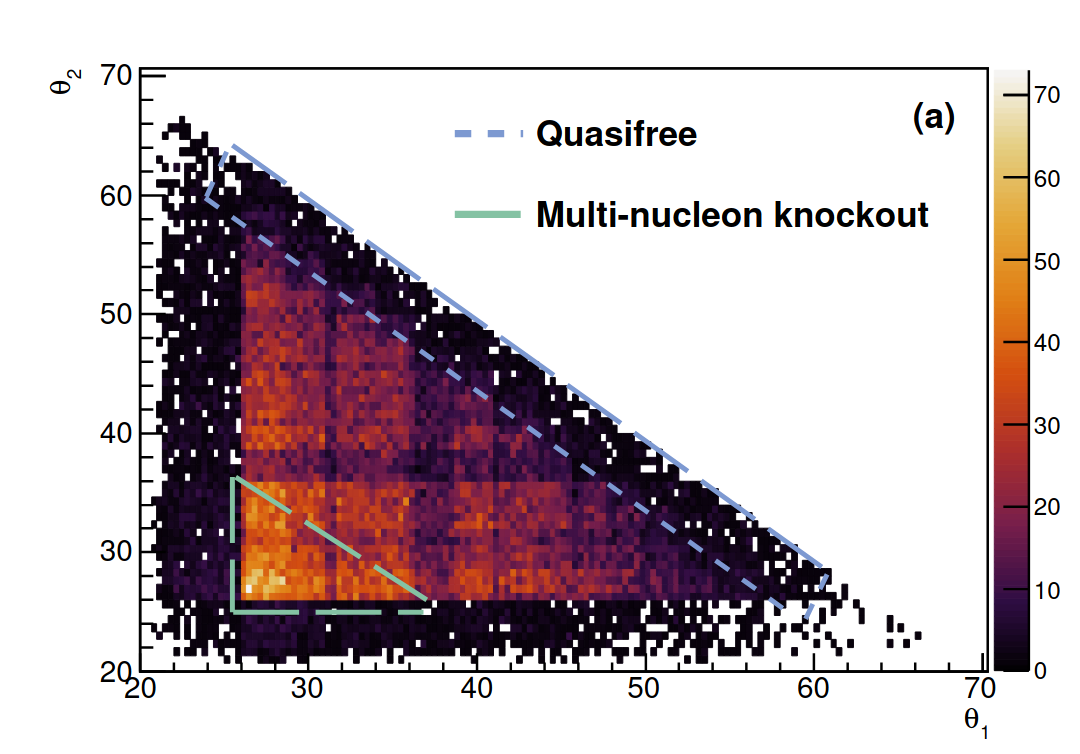
\includegraphics[width=\textwidth]{Figures/gabriel_1.png} 
    \end{subfigure}
    \begin{subfigure}[b]{0.3\textwidth}
    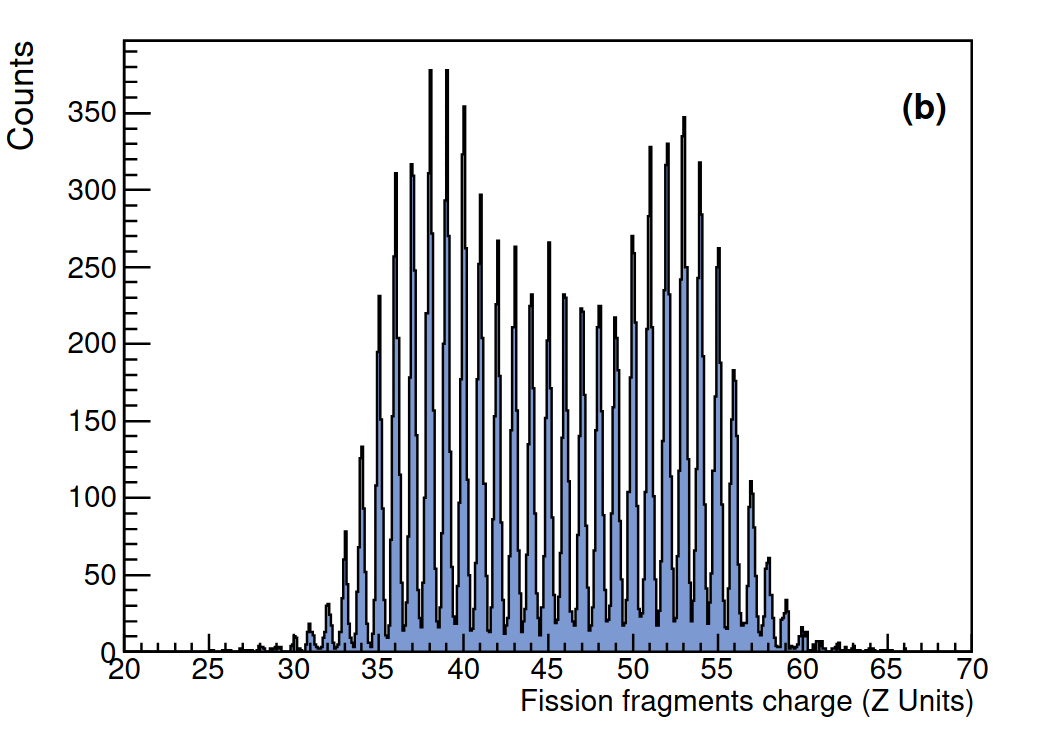
\includegraphics[width=\textwidth]{Figures/gabriel_2.png} 
    \end{subfigure}
    \begin{subfigure}[b]{0.3\textwidth}
    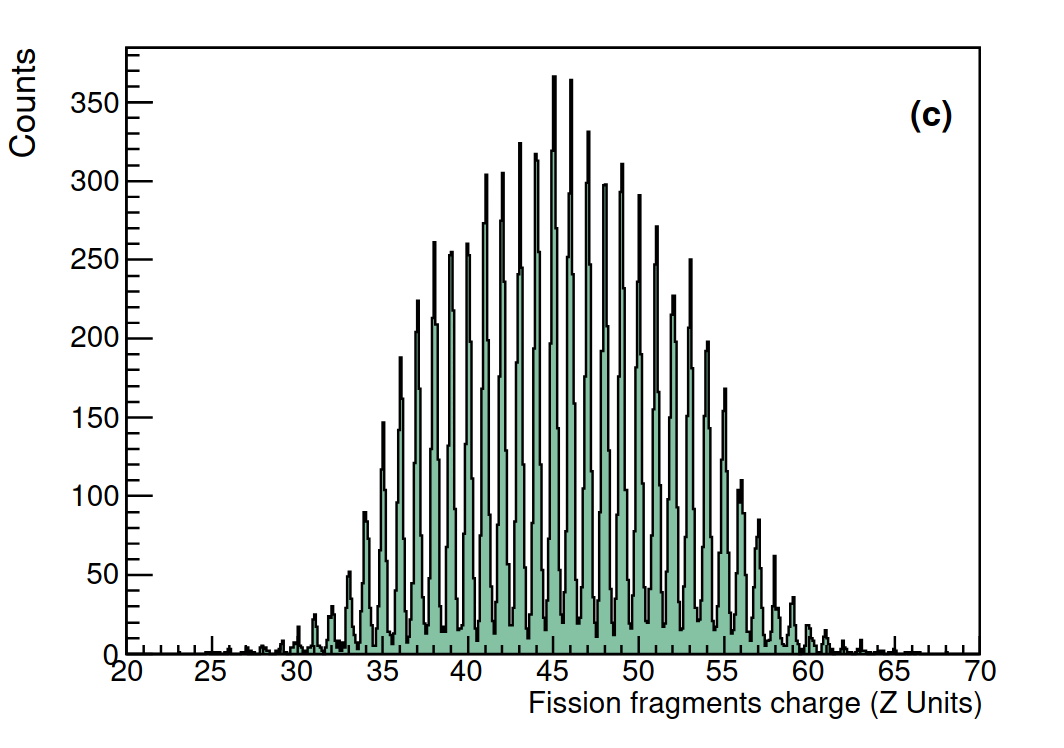
\includegraphics[width=\textwidth]{Figures/gabriel_3.png}
    \end{subfigure}
    \caption{(a) Polar angle correlations of the two protons from fission via QFS event. In (b)  the charge distribution for quasi-free (p,2p) fission reactions is selected while (c) displays the charge distribution for multi-nucleon knockout reactions of FSI. From Ref \cite{garcia2023study}, S455 Experiment in 2021 at R$^3$B, GSI.}
    \label{fig:qfs_fission}
\end{figure}
\newpage
The second part of the S455 experimental campaign employed a complementary and well-established method to investigate the fission process and its evolution: fission induced by Coulomb excitation (coulex-induced fission). This approach aimed at a precise characterization of fission yields and properties of 100 different neutron-deficient exotic isotopes, ranging from iridium (Z = 77) to thorium (Z = 90).\newline 
These isotopes were produced via the fragmentation of a relativistic  1 AGeV  $^{238}$U primary beam  and subsequently separated and identified individually using the GSI Fragment Separator (FRS). In the R$^3$B setup, the isotopes were directed onto a segmented lead target, where they were excited to a few MeV above their ground state energy, inducing the fission into two lighter fragments, which same as for the pilot fission via qfs experiment were identified and tracked within the dedicated R$^3$B detector setup.\newline
The systematic study of the data collected during ten days of experiment, revealed a transition toward increasingly asymmetric fission in neutron-deficient heavy nuclei This marks the discovery of a new “island of asymmetric fission” in the nuclear chart, characterized by a surprising dominance of light fission fragments with atomic number Z = 36, corresponding to krypton, see Fig.~\ref{fig:asymmetric_fission_islands}.\newline 
\begin{figure}[ht]
    \centering
    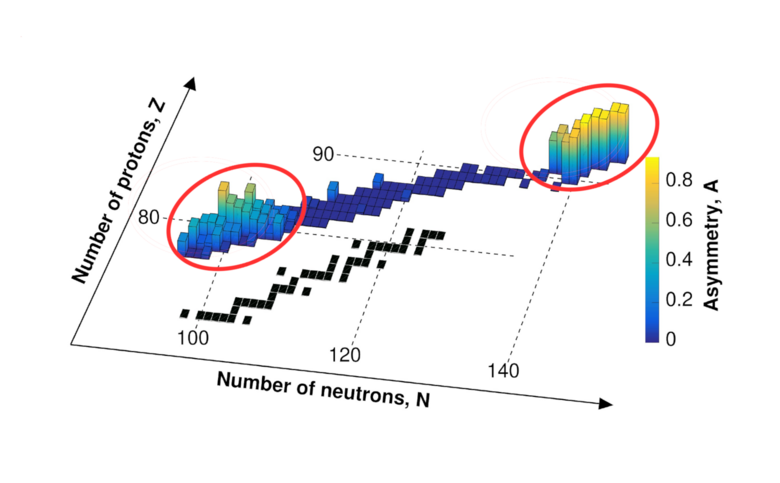
\includegraphics[width=0.85\textwidth]{Figures/csm_NuclideChart_with_islands_Foto_PMorfouace_res_47948441f0.png}
    \caption[Asymmetric fission regions in the chart of nuclides]{Three-dimensional chart of nuclides illustrating the evolution of asymmetric fission, with asymmetry \( A \) shown as a color scale. The red circles indicate two distinct regions—so-called ``islands''—of asymmetric fission. The region in the upper right corresponds to the well-established asymmetric fission in the actinide range (atomic numbers \( Z = 89\text{--}103 \)), where the process is stabilized by the formation of a heavy fragment near xenon (\( Z = 54 \)). In contrast, the region in the lower left highlights the recently discovered asymmetric fission of lighter nuclei around mercury (\( Z = 80 \)), stabilized by the formation of a light fragment near krypton (\( Z = 36 \)). Black squares denote the valley of beta-stable isotopes.\textit{Image credit: Pierre Morfouace, CEA, DAM, DIF, Arpajon, France.}}
    \label{fig:asymmetric_fission_islands}
\end{figure}
The significance of this discovery was underscored by its publication in Nature under the title \textit{“An asymmetric fission island driven by shell effects in light fragments”}~\cite{morfouace2025asymmetric}. This high-impact publication represents a major milestone for the R$^3$B collaboration and a notable recognition of the scientific importance of the experiment.\newline
This discovery marks a first step toward identifying the extent of a newly observed region in the nuclear chart where asymmetric fission dominates. A series of follow-up experiments is planned at FAIR, which will begin operation in 2027 within the “Early Science” campaign. At the heart of these efforts is the new Superconducting Fragment Separator (Super-FRS) -- the successor of the currently operating FRS -- a major upgrade that will enable the selection and delivery of even rarer and more exotic isotopes. These advancements will be key to mapping this phenomenon in much greater detail and revealing fundamental aspects of nuclear matter under extreme conditions.\newline

